% TJHSST CSL
% Writing Assignment
% Jonathan Lee

\documentclass[12pt]{article}
\usepackage{amsmath}
\usepackage{gensymb}
\usepackage{graphicx}
\usepackage{listings}
\usepackage{url}

% Horizontal spacing
\hoffset            0.00in
\oddsidemargin      0.00in
\evensidemargin     0.00in
\textwidth          6.50in
\marginparsep       0.00in
\marginparwidth     0.00in

% Vertical spacing
\voffset            0.00in
\topmargin          0.00in
\headheight         0.00in
\headsep            0.00in
\footskip           0.50in
\textheight         8.50in

\begin{document}
  \title{Validating Methods for Calculating Cosine}
  \author{Jonathan Lee}
  \date{November 9, 2015}
  \maketitle

  \abstract{
    Trigonometry forms the basis of all manner of fields, ranging from physics
    to geodesy. Therefore, an accurate and efficient method for calculating
    arbitrary trigonometric values is of great importance to many scientists
    and engineers. We sought to calculate the value of \(\cos(32 \degree)\) to
    test several techniques for calculating the cosine of an angle. Using a
    programming language cosine implementation, a weighted average, a continued
    fraction, and a series approximation, we estimated the value of \(\cos(32
    \degree)\) to be \(0.8480481\). The results of these technqiues show good
    agreement amongst themselves, and thus validate the accuracy of this
    quantity.
  }

  \section{Known Values}
    Using basic geometry, we can derive two values:
    \begin{equation}
      \begin{split}
        \cos(30 \degree) &= \frac{\sqrt{3}}{2} \\
          &= 0.866025404 \ldots
      \end{split}
    \end{equation}
    \begin{equation}
      \begin{split}
        \cos(36 \degree) &= \frac{1 + \sqrt{5}}{4} \\
          &= 0.80901699 \ldots
      \end{split}
    \end{equation}

  \section{An Unknown Value}
    To test our cosine calculations, we sought to find:
    \begin{align}
      \cos(32 \degree) = ?
    \end{align}

  \section{Calculations}
    \subsection{Programming Language Built-in Function}
      According to the R programming language \cite{R2015}, the value of
      {\tt{cos(32/180*pi)}} is \(0.8480481\), where {\tt{cos(x)}} takes an
      argument in radians.

    \subsection{Continued Fraction}
      Wolfram Alpha \cite{wolframalpha2015} gives:
      $$
      a = [0; 1, 5, 1, 1, 2, 1, 1, 2, 2, 3, 7, 4, 1, 6, 2, 1, 11, 2, 10, 2, 7,
        1, 1, 1, 7, 127, ...]
      $$
      as the first \(N\) terms of the continued fraction of \(\cos(32
      \degree)\). These terms can then be used to approximate the cosine as:

      \begin{align}
        \cos(x) = a_0 + \dfrac{1}{a_1 + \dfrac{1}{\ddots + \dfrac{1}{a_n}}}
      \end{align}

      The error of an approximation was calculated as:
      \begin{align}
        error = \frac{|expected - actual|}{expected} \times 100\%
      \end{align}

      As shown, the greater the number of terms, the closer the value
      approximates the expected value found using the cosine implementation of
      R:
      \begin{center}
        \begin{tabular}{|c||c|c|}
          \hline
          Terms & Value & Error (\%) \\
          \hline
          1 & 1.000000 & 17.917840 \\
          2 & 0.833333 & 1.735133 \\
          3 & 0.857143 & 1.072435 \\
          : & : & : \\
          N & 0.848048 & 0.000000 \\
          \hline
        \end{tabular}
      \end{center}
      \begin{center}
        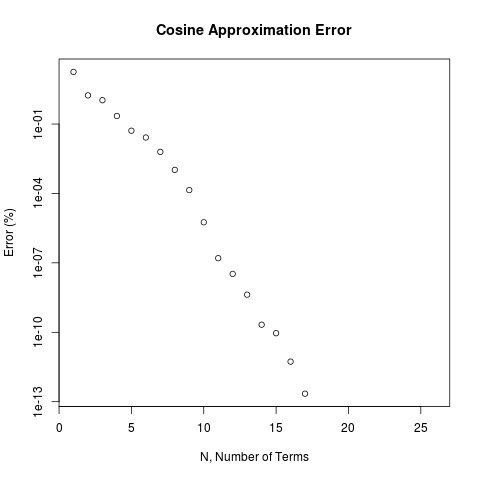
\includegraphics[width=0.5\textwidth]{error}
      \end{center}

    \subsection{Simple Average}
      If we assume \(\cos(x)\) approximates a linear function near
      \(x = 32 \degree\), then we can simply take a weighted average of values
      close to the x-coordinate.
      \begin{equation}
        \begin{split}
          \cos(x) &= \frac{4\cos(30 \degree) + 2\cos(36 \degree)}{6} \\
            &= \frac{\sqrt{3} + \left(\frac{1 + \sqrt{5}}{4}\right)}{3} \\
            &= \frac{\sqrt{3}}{3} + \frac{1 + \sqrt{5}}{12} \\
            &= 0.8470226006479417 \ldots
        \end{split}
      \end{equation}

    \subsection{Series Approximation}
      Using a commonly used Taylor series \cite{taylorseries2015}, we can
      approximate the value of \(\cos(32 \degree)\):
      \begin{equation}
        \begin{split}
          \cos(x) &= 1 - \frac{x^2}{2!} + \frac{x^4}{4!} - \frac{x^6}{6!} +
              \frac{x^8}{8!} - \ldots \\
            &= \sum_{i=0}^{\infty} (-1)^{i} \frac{x^{2i}}{(2i)!}
        \end{split}
      \end{equation}
      \begin{align}
        \cos(32 \degree) = 0.848048096156426 \ldots
      \end{align}

    \subsection{Other Ideas}
      To find \(\cos(32 \degree)\), we could also approximate the value
        graphically.

  \section{Conclusion}
    With the exception of the weighted average, each method produced a value
    for \(\cos(32 \degree)\) within at least three decimal places of each
    other. The weighted average is an outlier because it is not a precise
    approximation, and to improve this method, we would have to take values for
    cosine closer to \(x = 32 \degree\). Thus, we have shown the other three
    methods can calculate cosine within an acceptable range of error. In the
    future, further work could focus on graphical approximation methods.

  \pagebreak

  \bibliography{writing}
  \bibliographystyle{plain}
\end{document}
